\chapter{System Usage}

\section{Communication Server}

The setup enabled the server to start automatically with the jetson, so after installation be sure to restart your device.

\section{ User Application }
See figure below:
\begin{figure}[h!]
	\centering
	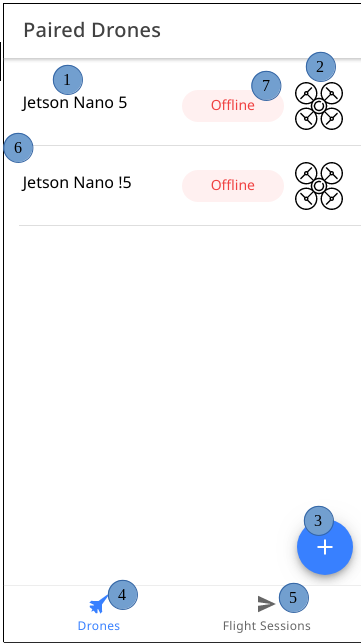
\includegraphics[scale=0.5]{./assets/images/offline.png}
	\label{fig: screens}
	\caption{}
\end{figure}
\begin{itemize}
		\item 1. Drone name.
		\item 2. Drone icon
		\item 3. Navigate to 'add new drone' page.
		\item 4. Navigate to drone list tab
		\item 5. Navigate to flight sessions tab
		\item 6. Drones list
		
\end{itemize}
\begin{figure}[h!]
	\centering
	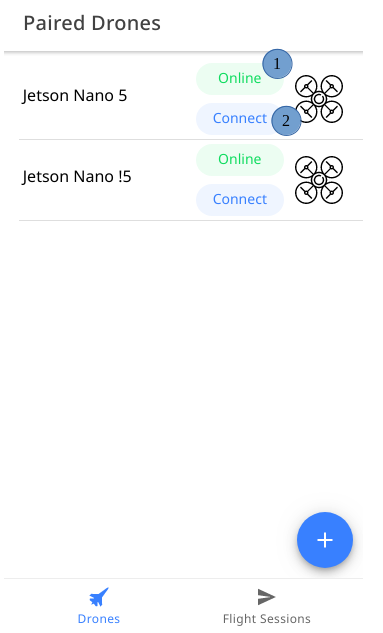
\includegraphics[scale=0.5]{./assets/images/online.png}
	\label{fig: screens}
	\caption{}
\end{figure}
\newpage
\begin{itemize}
		\item 1. Server status online
		\item 2. Connect to drone/server button
\end{itemize}

\begin{figure}[h!]
	\centering
	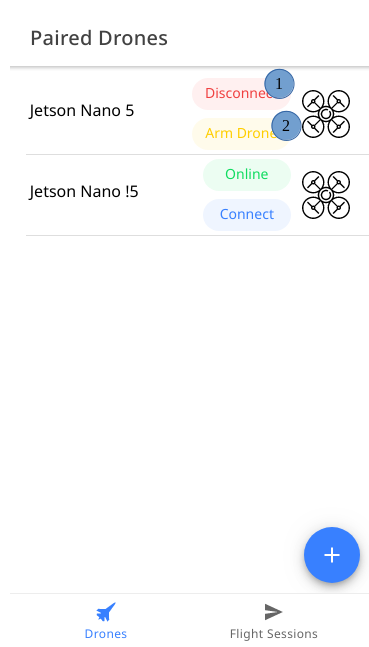
\includegraphics[scale=0.5]{./assets/images/connected.png}
	\label{fig: screens}
	\caption{}
\end{figure}
\newpage
\begin{itemize}
		\item 1. Disconnect drone button.
		\item 2. Arm drone button.
\end{itemize}


